\section{Experiments}

  For a variety of CPUs, we benchmarked the convolutional layers of
  several state-of-the-art ConvNets used for (1) 2D object detection,
  (2) 2D image segmentation, and (3) 3D spatiotemporal feature
  learning.

  \begin{table} \centering
    \setlength\tabcolsep{2.5pt}
    \begin{tabular}{cr !{\vrule width0.8pt} cccccc  }
      &  & B & F & F' & Image Size & Padding & Kernel Size  \\
      \hline
      \multirow{5}{*}{\rotatebox{90}{\textbf{VGG-a}}}
      & C2 & 64  & 64  &  128 & $\angled{112,112}$ & $\angled{1,1}$ & $\angled{3,3}$ \\
      & C3 & 64  & 128 &  256 & $\angled{56,56}$   & $\angled{1,1}$ & $\angled{3,3}$ \\
      & C4 & 64  & 256 &  256 & $\angled{56,56}$   & $\angled{1,1}$ & $\angled{3,3}$ \\
      & C5 & 64  & 256 &  512 & $\angled{28,28}$   & $\angled{1,1}$ & $\angled{3,3}$ \\
      & C6 & 64  & 512 &  512 & $\angled{28,28}$   & $\angled{1,1}$ & $\angled{3,3}$ \\
      \hline
      \multirow{5}{*}{\rotatebox{90}{\textbf{U-Net}}}
      & C1b & 1  & 64  &  64 & $\angled{570,570}$  & $\angled{0,0}$ & $\angled{3,3}$ \\
      & C2b & 1  & 128 &  128 & $\angled{282,282}$ & $\angled{0,0}$ & $\angled{3,3}$ \\
      & C3b & 1  & 256 &  256 & $\angled{138,138}$ & $\angled{0,0}$ & $\angled{3,3}$ \\
      & C4b & 1  & 512 &  512 & $\angled{66,66}$   & $\angled{0,0}$ & $\angled{3,3}$ \\
      & C5b & 1  & 1024 &  1024 & $\angled{30,30}$ & $\angled{0,0}$ & $\angled{3,3}$ \\
      \hline
      \multirow{5}{*}{\rotatebox{90}{\textbf{C3D}}}
      & C2a & 32  & 64  &  128 & $\angled{16,56,56}$ & $\angled{1,1,1}$ & $\angled{3,3,3}$ \\
      & C3a & 32  & 128 &  256 & $\angled{8,28,28}$ & $\angled{1,1,1}$ & $\angled{3,3,3}$ \\
      & C3b & 32  & 256 &  256 & $\angled{8,28,28}$ & $\angled{1,1,1}$ & $\angled{3,3,3}$ \\
      & C4a & 32  & 256 &  512 & $\angled{4,14,14}$ & $\angled{1,1,1}$ & $\angled{3,3,3}$ \\
      & C4b & 32  & 512 &  512 & $\angled{4,14,14}$ & $\angled{1,1,1}$ & $\angled{3,3,3}$ \\
      \hline
      \multirow{5}{*}{\rotatebox{90}{\textbf{Toy}}}
      & 2D1 & 64  & 48 &  96 & $\angled{114,114}$ & $\angled{0,0}$ & $\angled{3,3}$ \\
      & 2D2 & 64  & 48 &  96 & $\angled{58,58}$ & $\angled{0,0}$ & $\angled{5,5}$ \\
      & 2D3 & 64  & 48 &  96 & $\angled{58,58}$ & $\angled{0,0}$ & $\angled{11,11}$ \\
      & 3D1 & 32  & 48 &  96 & $\angled{10,30,30}$ & $\angled{0,0}$ & $\angled{2,3,3}$ \\
      & 3D2 & 32  & 48 &  96 & $\angled{10,20,20}$ & $\angled{0,0}$ & $\angled{3,5,5}$ \\
      \hline
    \end{tabular}
    \caption{Benchmarked convolutional layers.}
    \label{table:layers}
  \end{table}

  \begin{table}
    \begin{center}
      \setlength\tabcolsep{2.5pt}
      \begin{tabular}{lrrrr}
        \toprule
        CPU & Frequency & CPUs $\times$ Cores/Threads & GFLOPS\\
        \midrule
        i7-6700K (Skylake) & 4GHZ & 1 $\times$ 4/8 & 512\\
        $4\times$ E7-8890v3 (Haswell) & 2.5GHz & 4 $\times$ 18/36 & 5760\\
        Xeon Phi 7210 & 1.1GHz & 1 $\times$ 64/256 & 4505.6\\
        \toprule
        GPU & Frequency & CUDA cores & GFLOPS\\
        \midrule
        Titan X (Maxwell) & 1GHz & 3072 & 6600\\
        Titan X (Pascal) & 1.5GHz & 3584  &  11000\\
        \bottomrule
      \end{tabular}
    \end{center}
    \caption{CPUs and GPUs used for benchmarks.}
    \label{table:cpus}
  \end{table}

  The 2D object detection ConvNet was the VGG-A version of
  OxfordNet~\cite{simonyan2014very}, an
  ImageNet~\cite{imagenet_cvpr09,ILSVRC15} winner that is widely used
  for speed benchmarks~\cite{imagenetwinners}.  The 2D image
  segmentation ConvNet was U--Net~\cite{ronneberger2015u}, used for
  biomedical image segmentation.  The object detection network uses
  ``batch training'' (multiple sets of inputs at the time), and
  gradually downsampled images.  The segmentation network uses rather
  large images with $B=1$.  The 3D spatiotemporal feature learning
  network was C3D~\cite{maturana_iros_2015}.  For each network, we
  benchmarked the five most computationally expensive convolutional
  layers (Table~\ref{table:layers}).

  The above ConvNets use only kernel sizes of $3 \times 3$ or $3\times
  3\times 3$, and the number of images in a layer is always a power of
  two.  To make our benchmarks more general (see ``Toy'' of
  Table~\ref{table:layers}), we also include layers with kernel sizes
  $5 \times 5$ and $11 \times 11$, inspired by
  AlexNet~\cite{krizhevsky2012imagenet}, kernel size $2 \times 3
  \times 3$, inspired by VD2D3D~\cite{lee2015recursive}, and kernel
  size $3 \times 5 \times 5$.  We also include layers with number of
  images not equal to a power of two.

  In addition, we benchmark each layer on three generations
  of Intel Xeon processors (Table~\ref{table:cpus}).  All the machines
  except the Skylake CPU were set to run at constant frequency (we did
  not have root access to the Skylake machine).

  \begin{figure*} \centering
    \small
    \setlength\tabcolsep{0.5pt}
    \begin{tabular}{ >{\centering\arraybackslash}c ccccccl }
      \toprule
      & \multicolumn{2}{c}{\textbf{Skylake}}
      & \multicolumn{2}{c}{\textbf{Haswell}}
      & \multicolumn{2}{c}{\textbf{Knights Landing}} & \\
      \midrule
      & Forward & Update & Forward & Update & Forward & Update & \\
      \midrule
      \rotatebox{90}{\qquad \textbf{VGG-A}}
      & 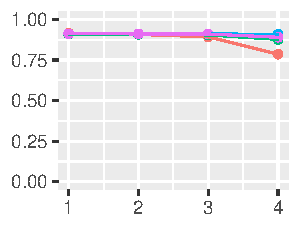
\includegraphics[height=2.4cm]{fig/vgg-fwd-skylake}
      & 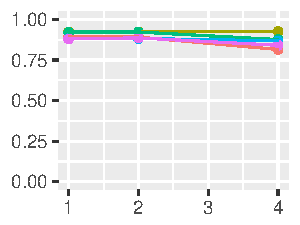
\includegraphics[trim=8mm 0mm 0mm 0mm,clip,height=2.4cm]{fig/vgg-upd-skylake}
      & 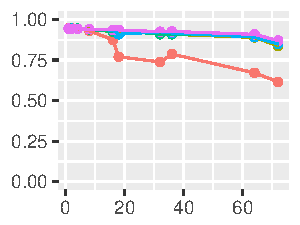
\includegraphics[trim=8mm 0mm 0mm 0mm,clip,height=2.4cm]{fig/vgg-fwd-haswell}
      & 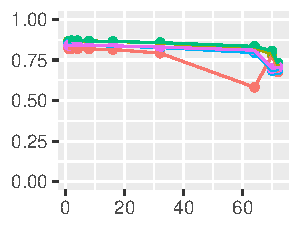
\includegraphics[trim=8mm 0mm 0mm 0mm,clip,height=2.4cm]{fig/vgg-upd-haswell}
      & 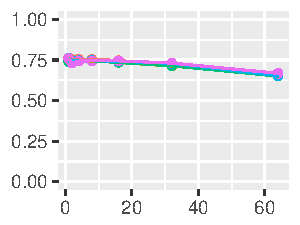
\includegraphics[trim=8mm 0mm 0mm 0mm,clip,height=2.4cm]{fig/vgg-fwd-knl}
      & 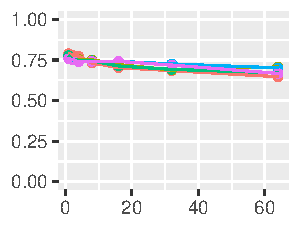
\includegraphics[trim=8mm 0mm 0mm 0mm,clip,height=2.4cm]{fig/vgg-upd-knl}
      & 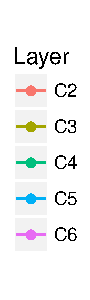
\includegraphics[height=2.4cm]{fig/vgg-legend} \\
      \midrule
      \rotatebox{90}{\qquad \textbf{U-Net}}
      & 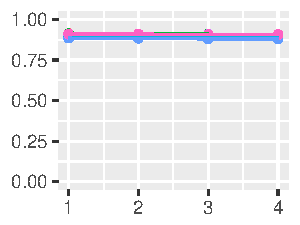
\includegraphics[height=2.4cm]{fig/unet-fwd-skylake}
      & 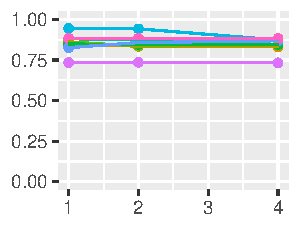
\includegraphics[trim=8mm 0mm 0mm 0mm,clip,height=2.4cm]{fig/unet-upd-skylake}
      & 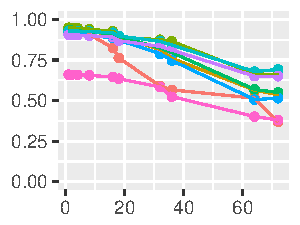
\includegraphics[trim=8mm 0mm 0mm 0mm,clip,height=2.4cm]{fig/unet-fwd-haswell}
      & 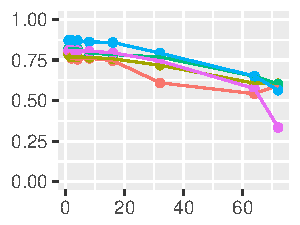
\includegraphics[trim=8mm 0mm 0mm 0mm,clip,height=2.4cm]{fig/unet-upd-haswell}
      & 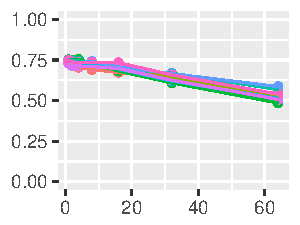
\includegraphics[trim=8mm 0mm 0mm 0mm,clip,height=2.4cm]{fig/unet-fwd-knl}
      & 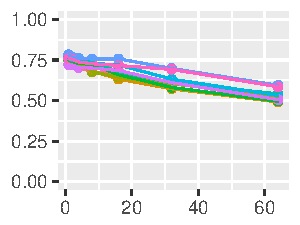
\includegraphics[trim=8mm 0mm 0mm 0mm,clip,height=2.4cm]{fig/unet-upd-knl}
      & 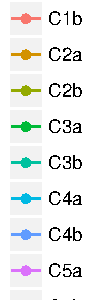
\includegraphics[height=2.4cm]{fig/unet-legend} \\
      \midrule
      \rotatebox{90}{\qquad \textbf{C3D}}
      & 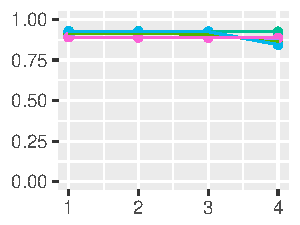
\includegraphics[height=2.4cm]{fig/d3d-fwd-skylake}
      & 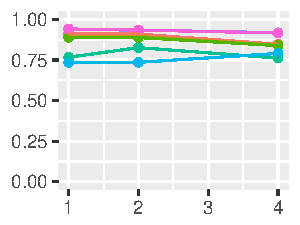
\includegraphics[trim=8mm 0mm 0mm 0mm,clip,height=2.4cm]{fig/d3d-upd-skylake}
      & 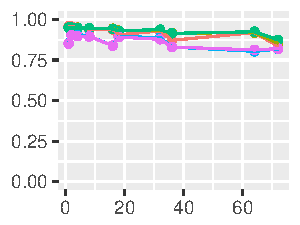
\includegraphics[trim=8mm 0mm 0mm 0mm,clip,height=2.4cm]{fig/d3d-fwd-haswell}
      & 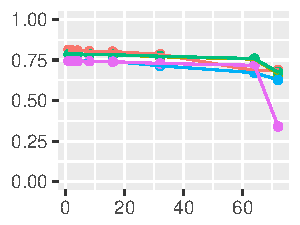
\includegraphics[trim=8mm 0mm 0mm 0mm,clip,height=2.4cm]{fig/d3d-upd-haswell}
      & 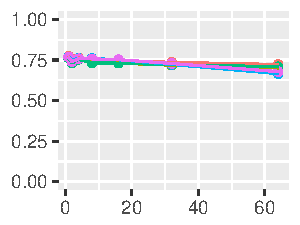
\includegraphics[trim=8mm 0mm 0mm 0mm,clip,height=2.4cm]{fig/d3d-fwd-knl}
      & 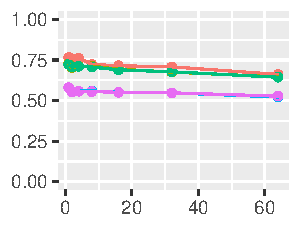
\includegraphics[trim=8mm 0mm 0mm 0mm,clip,height=2.4cm]{fig/d3d-upd-knl}
      & 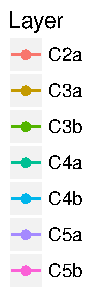
\includegraphics[height=2.4cm]{fig/d3d-legend} \\
      \midrule
      \rotatebox{90}{\qquad \textbf{Toy}}
      & 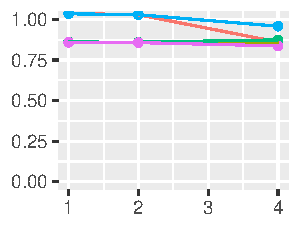
\includegraphics[height=2.4cm]{fig/toy-fwd-skylake}
      & 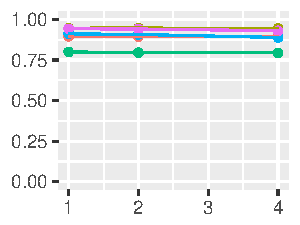
\includegraphics[trim=8mm 0mm 0mm 0mm,clip,height=2.4cm]{fig/toy-upd-skylake}
      & 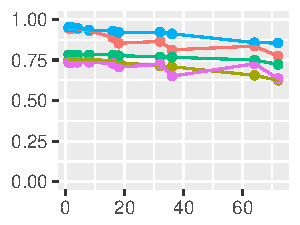
\includegraphics[trim=8mm 0mm 0mm 0mm,clip,height=2.4cm]{fig/toy-fwd-haswell}
      & 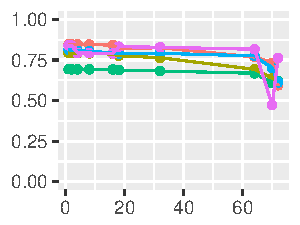
\includegraphics[trim=8mm 0mm 0mm 0mm,clip,height=2.4cm]{fig/toy-upd-haswell}
      & 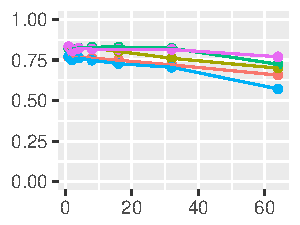
\includegraphics[trim=8mm 0mm 0mm 0mm,clip,height=2.4cm]{fig/toy-fwd-knl}
      & 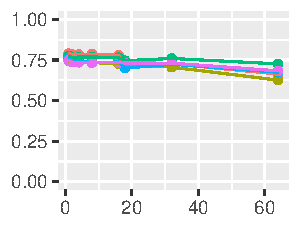
\includegraphics[trim=8mm 0mm 0mm 0mm,clip,height=2.4cm]{fig/toy-upd-knl}
      & 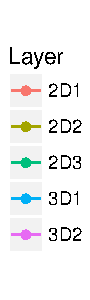
\includegraphics[height=2.4cm]{fig/toy-legend} \\
      \bottomrule

    \end{tabular}
    \caption{Utilization and scalability of our algorithms across
      different layers and CPU generations.  The $x$--axis represent
      number of cores used.  The $y$ axis represents the percentage of
      utilization of the used cores.}
    \label{fig:scalability}
  \end{figure*}

  \subsection{Benchmarking methodology}

  We benchmark both the propagation and the update algorithm for each
  layer on each CPU in the following way.  We compile the full layer
  primitive such that it uses only $N$ of the available cores and $H$
  hyper--threads per core.  We then perform 10 iterations of (1)
  randomly initializing all the data and (2) running the algorithm.
  We report the average time of running the second step.

  Randomly initializing the data before each iteration is important,
  as it clears the CPU caches.  Thus, our measurements represent a
  lower bound on the time required when the layer is part of a larger
  network that is being trained.  The speed of each primitive is
  computed by dividing the FLOPs required for the algorithm by
  average runtime.  The utilization is computed by dividing the speed
  of our algorithm (in FLOPS) by the FLOPS deliverable by $N$ cores of
  the given CPU.

  For Skylake and Haswell, we benchmarked our algorithm
  using gcc-5.3, icc-16 and clang-3.9.  The measured times were within
  a couple of percent, with icc-16 being the slowest, and clang-3.9
  being the fastest.  We report the gcc-5.3 numbers.

  For Xeon Phi, icc-16 and clang-3.9 performed equally well, with
  gcc-5.3 greatly under--performing.  Upon examining the generated
  assembly code, we noticed that gcc-5.3 failed to use the
  scalar--vector FMA instructions available.  The numbers reported are
  for icc-16.

  \subsection{CPU utilization and scalability}

  Utilization and scalability are shown in Fig~\ref{fig:scalability}.
  The $x$ axis represents the number of cores used, and the $y$ axis
  represents the percentage of utilization of the used cores.  A
  horizontal line would mean perfectly linear scalability.  For
  simplicity, points are only shown for the optimal number
  of hyper--threads per core, which was $2$ in more than 90\% of cases.

  Theoretically, more hyper--threads per core can hide memory latency,
  but will reduce effective cache sizes and might introduce cache
  associativity conflicts.  In practice, many factors such as blocking
  size, kernel sizes, available cache, etc...  come in play.  For this
  reason, it is the best to empirically determine the optimal choice.

  In nearly all cases, single core utilization is higher than 75\%.
  As we were unable to limit the CPU frequency on the Skylake CPU used
  for benchmarks, the turbo--boost that was enabled resulted in
  utilization higher than 100\% when one or two cores out of four
  available were used.

  Fig.~\ref{fig:scalability} suggest that our algorithms scale very
  well, with near linear scalability even for the multi--chip Haswell
  system.

  With relatively small number of cores, the Skylake machine has both
  high utilization for the serial algorithm, and linear scalability.
  Both Skylake and Haswell had higher utilization for the serial
  algorithm (1 core used).  Non--optimal ordering of vector
  instructions, not enough loop unrolling, as well as lack of L3 cache
  all contributed to lower CPU utilization.  While we expect the first
  two problems to be solved as compilers for KNL mature, we still
  expect a CPU with L3 cache to somehow outperform ones without it.

  On the other side, we notice that the scalability is relatively
  worse for the case of U--Net, which can be considered a hard case.
  This is because the total amount of computation required by U--Net
  layers is relatively small, thus, even a single synchronization
  point will affect the scalability.  This is especially pronounced
  for the Haswell machine with 4 NUMA nodes.  Another reason for
  relatively lower scalability is the fact that U--Net's batch size of
  $1$ yields a subdivision into non--exactly--equal size problems.

  \subsection{Comparison versus other CPU implementations}

  We compare the speed of our approach to several competing CPU
  implementations for 2D ConvNets, CcT~\cite{hadjis2015shallow},
  MKL--DNN and MKL--2017.  We used the CcT version of Caffe for CcT,
  as well as the latest Intel--Caffe fork~\footnote{as of November
    2017} for MKL-DNN and MKL-2017.  MKL-DNN provides only optimized
  primitives for AVX2 and forward/backward propagation, and would
  fallback to Caffe's default gemm method for other primitives.  Caffe
  benchmarks report the cumulative time of the backward propagation
  and update phase, so we report the numbers of our approach in the
  same fashion.  This is reasonable as in practice the backward pass
  and update phase are always performed one after the other.

% We are unable to compare the speed against
%  ZNN~\cite{zlateski2016znn} as it doesn't support layer--wise
%  computation, but rather parallelizes the whole training algorithm.
%  Also, we don't expect ZNN to be competitive as it is optimized for
%  large kernels.



  \begin{table} \centering
    \setlength\tabcolsep{2.5pt}
    \begin{tabular}{cr !{\vrule width0.8pt} rr|rr|rr|rr  }
      & & \multicolumn{2}{c|}{MKL-DNN} & \multicolumn{2}{c|}{MKL-2017}
      & \multicolumn{2}{c|}{CcT} & \multicolumn{2}{c}{Ours} \\
      &  & Fwd & B+U & Fwd & B+U& Fwd & B+U& Fwd & B+U \\
      \hline
      \multirow{5}{*}{\rotatebox{90}{\textbf{VGG-A}}}
      & C2  & 79.1  & 196.4 & 43.8 & 99.3  & 141.2 & 317.8 & {\bf 33.4} & {\bf 60.4}  \\
      & C3  & 42.4  & 106.8 & 30.0 & 78.5  & 118.5 & 194.3 & {\bf 24.5} & {\bf 60.3}  \\
      & C4  & 101.3 & 322.3 & 58.6 & 158.0 & 263.5 & 395.4 & {\bf 48.2} & {\bf 100.6} \\
      & C5  & 44.2  & 203.5 & 27.3 & 76.2  & 92.6  & 233.9 & {\bf 24.2} & {\bf 53.2}  \\
      & C6  & 89.8  & 466.5 & 54.8 & 149.9 & 196.8 & 466.3 & {\bf 47.2} & {\bf 104.2} \\
      \hline
      \multirow{5}{*}{\rotatebox{90}{\textbf{U-Net}}}
      & C1b  & 257.44 & 494.93 & 183.16 & 195.86 & 1739 &  542 & {\bf 9.02} & {\bf 18.12} \\
      & C2b  & 127.55 & 248.83 & 82.80  & 42.53  & 1052 & 1671 & {\bf 6.07} & {\bf 13.91} \\
      & C3b  & 66.17  & 126.35 & 38.48  & 25.20  & 2988 & 4645 & {\bf 5.47} & {\bf 13.41} \\
      & C4b  & 53.89  & 90.54  & 18.66  & 26.90  & 2172 & 4033 & {\bf 5.16} & {\bf 13.21} \\
      & C5b  & 19.34  & 77.86  & 9.24   & 22.09  & 1667 & 3198 & {\bf 4.35} & {\bf 11.23} \\
      \hline

    \end{tabular}
    \caption{Benchmarks of the 2D layers against CcT, MKL-DNN and
      MKL-2017 on the 4--way E7-8890v3 (Haswell) machine.}
    \label{table:2d-haswell}
  \end{table}

  On a 4--way Haswell machine, MKL--2017 was the best of the three
  competitors (Table~\ref{table:2d-haswell}), and our approach
  outperformed MKL--2017.  For VGG--A layers, MKL--2017 was not much
  slower (only 10-20\% for forward propagation, and 50\% for backward
  propagation + update).  For U-Net layers, our approach greatly
  outperformed MKL--2017, with up to $20\times$ greater speed
  for layer $C1b$ forward propagation.

  \begin{table} \centering
    \setlength\tabcolsep{2.5pt}
    \begin{tabular}{cr !{\vrule width0.8pt} rr|rr|rr  }
      & & \multicolumn{2}{c|}{MKL-DNN} & \multicolumn{2}{c|}{MKL-2017}
      & \multicolumn{2}{c}{Ours} \\
      &  & Fwd & B+U& Fwd & B+U& Fwd & B+U \\
      \hline
      \multirow{5}{*}{\rotatebox{90}{\textbf{VGG-A}}}
      & C2  & 101.9 & 266.8 & {\bf 34.6} & 101.8 & 40.1 & {\bf  80.7}  \\
      & C3  & 72.5  & 192.3 & {\bf 32.9} & 87.1  & 39.7 & {\bf  76.8}  \\
      & C4  & 142.0 & 402.9 & {\bf 65.4} & 166.2 & 80.6 & {\bf 158.9}  \\
      & C5  & 53.0  & 268.5 & {\bf 32.8} & {\bf 72.9}  & 40.1 & 77.5   \\
      & C6  & 108.3 & 557.3 & {\bf 64.8} & 172.3 & 78.6 & {\bf 157.3}  \\
      \hline
      \multirow{5}{*}{\rotatebox{90}{\textbf{U-Net}}}
      & C1b  & 799.60 & 1603.93 & 141.01 & 61.96 & {\bf 9.89} & {\bf 21.81} \\
      & C2b  & 382.60 & 790.76  & 48.93  & 23.27 & {\bf 9.79} & {\bf 20.31} \\
      & C3b  & 187.08 & 421.61  & 23.10  & 16.84 & {\bf 8.50} & {\bf 16.71} \\
      & C4b  & 94.81  & 259.73  & 10.56  & 24.70 & {\bf 7.31} & {\bf 15.49} \\
      & C5b  & 44.01  & 167.88  & {\bf 5.45}   & {\bf 10.84} & 6.01 & 12.33 \\
      \hline

    \end{tabular}
    \caption{Benchmarks of the 2D layers against MKL-DNN and MKL-2017
      on the Xeon Phi 7210 machine.  CcT was not included as it did not compile for Xeon Phi.}
    \label{table:2d-knl}
  \end{table}

  For Xeon Phi, our approach was comparable to MKL-2017 for VGG-A
  layers, with MKL-2017 having a slight edge
  (Table~\ref{table:2d-knl}).  For U--Net layers, our approach was far
  superior to MKL-2017 on layers with fewer images, and was only
  slightly inferior on the widest layer with 1024 images.

  To summarize, our approach is far superior to competitors for
  training image segmentation architectures like U-Net.  For object
  detection architectures like VGG-A, our approach is slightly
  inferior to MKL-2017 for Xeon Phi KNL and slightly superior for
  4--way Haswell.

  \section{CPU vs. GPU for 3D convolutional layers}
  While the CPU performance numbers given above are encouraging, they
  still fall short of GPU performance numbers.  This is partially
  because a state-of-the-art GPU has $2\times$ the FLOPS of a
  state-of-the-art CPU (Table \ref{table:cpus}).  It is also because
  cuDNN is highly optimized and often achieves extremely high
  percentage utilization of available FLOPS.  This is especially the
  case with popular benchmark architectures for object detection like
  VGG-A.  Utilization is somewhat less for segmentation networks like
  U-Net (data not shown).

  However, it turns out that our approach is competitive with GPUs for
  3D convolutional layers.  For the comparison of Table
  \ref{eq:GPUvsCPU}, we used direct cuDNNv5 calls from C++, and the
  two latest generations of the Titan X GPU.  Surprisingly, our
  approach applied to the 4--way Haswell machine gives performance
  comparable to the Titan X Pascal.  This means that for 3D ConvNets
  our approach can compensate for the lower theoretical FLOPS of the
  Haswell machine (Table \ref{table:cpus}) by achieving higher
  percentage utilization.


  \begin{table} \centering
    \setlength\tabcolsep{2.5pt}
    \begin{tabular}{cr !{\vrule width0.8pt} rr|rr !{\vrule width0.8pt} rr|rr  }
      & & \multicolumn{4}{c !{\vrule width0.8pt} }{\textbf{cuDNNv5 (Titan X)}} & \multicolumn{4}{c}{\textbf{Ours (Xeon)}} \\
      & & \multicolumn{2}{c|}{Maxwell} & \multicolumn{2}{c!{\vrule width0.8pt}}{Pascal}
      & \multicolumn{2}{c|}{Haswell} & \multicolumn{2}{c}{KNL} \\
      &  & Fwd & B+U & Fwd & B+U& Fwd & B+U& Fwd & B+U \\
      \hline
      \multirow{5}{*}{\rotatebox{90}{\textbf{C3D}}}
      & C2a & 186.8 & 370.3 & 168.0 & 336.0 & {\bf 147.6} & {\bf 325.2} & 218.1 & 456.3  \\
      & C3a & 90.1  & 180.0 & 78.5  & {\bf 161.2} & {\bf 72.2}  & 162.9 & 112.3 & 234.3  \\
      & C3b & 178.0 & 359.5 & 153.0 & 310.0 & {\bf 141.0} & {\bf 308.1} & 222.4 & 467.1  \\
      & C4a & 32.8  & 68.7  & 28.3  & {\bf 59.6}  & {\bf 27.7}  & 63.1  & 43.4  &  98.8  \\
      & C4b & 65.1  & 135.1 & 55.7  & {\bf 117.4} & {\bf 55.2}  & 131.2 & 85.3  & 196.1  \\
      \hline
    \end{tabular}
    \caption{GPU vs. CPU for 3D convolutional layers}
    \label{eq:GPUvsCPU}
  \end{table}
